Une matrice $A\in \mathcal{M}_n(\R)$ admet une \emph{décomposition de Cholesky} si et seulement si il existe une matrice $U\in \mathcal{M}_n(\R)$ triangulaire supérieure et inversible telle que $A = \trans U U$. Cette expression est appelée la \emph{décomposition de Cholesky} de $A$.
\subsection*{Partie I. Algorithme 1.}
On suppose que $A\in \mathcal{M}_n(\R)$ admet une décomposition de Cholesky $A= \trans U U$ où $U$ est une matrice triangulaire supérieure \emph{dont tous les termes diagonaux sont strictement supérieurs à} $0$.
\begin{enumerate}
 \item Montrer que $A$ est symétrique.
 \item Compléter la caractérisation suivante:
\begin{displaymath}
U \text{ triangulaire supérieure } \Leftrightarrow \left( \forall (i,j)\in \llbracket 1,n \rrbracket^2, \;\phantom{i > j}\; \Rightarrow u_{i j} = 0 \right) 
\end{displaymath}
 \item Montrer que $\forall j \in  \llbracket 1,n \rrbracket, \hspace{0.5cm} u_{1 1}u_{1 j} = a_{1 j}$.
 \item Montrer que $\forall i \in \llbracket 2,n \rrbracket,\; \forall j \in \llbracket i, n \rrbracket,\hspace{0.5cm}  \sum_{k = 1}^{i} u_{k i} u_{k j} = a_{i j}$.
En déduire 
\begin{displaymath}
 \forall i \in \llbracket 2,n \rrbracket,\; \forall j \in \llbracket i, n \rrbracket,\hspace{0.5cm}
 \sum_{k = 1}^{i-1} u_{k i} u_{k j} + u_{i i} u_{i j} = a_{i j}
\end{displaymath}
\item Compléter l'algorithme \ref{Echolesky_1} qui permet de calculer la matrice $U$ à partir de $A$. On supposera que la matrice $A$ est \emph{définie positive} c'est à dire telle que les expressions qui figurent sous les racines carrées sont strictement positives.
\begin{algorithm}
  $n\leftarrow $ naturel non  nul\;
  $A\leftarrow $ matrice $n\times n$ définie positive \;
  $U$ désigne la matrice triangulaire supérieure que l'on veut calculer \;
  $i\leftarrow 1$\;
  $u_{1 1} \leftarrow \sqrt{\,??\, }$\;
  \Pour{$j$ de $2$ à $n$:}{
    $u_{1 j} \leftarrow \frac{??}{u_{1 1}}$
  }
  \Pour{$i$ de $2$ à $n$}{
      $u_{i i} \leftarrow \sqrt{\,??\, }$\;
    \Pour{$j$ de $i+1$ à $n$:}{
      $u_{i j} \leftarrow \frac{??}{u_{i i}}$
    }
  }
  \caption{Partie I. Question 5}
  \label{Echolesky_1}
\end{algorithm}

\end{enumerate}

\subsection*{Partie II. Application aux systèmes.}
Dans cette partie, les matrices seront représentées en Python par des listes de listes.
 Exemple
 \begin{align*}
\begin{pmatrix}
 1 & 2 & 3 \\ 5 & 1 &-1
\end{pmatrix}
\text{ représenté par }& \texttt{[[1,2,3],[5,1,-1]]} \\
\begin{pmatrix}
 2 \\ 3 \\ 1
\end{pmatrix}
\text{ représenté par }& \texttt{[[2],[3],[1]]}
 \end{align*}
\begin{enumerate}
 \item Implémenter en pseudo-code la résolution d'un système $SX=Y$ où $S$ est une matrice triangulaire supérieure inversible $n\times n$ et $Y$ une matrice colonne.
 \item 
    \begin{enumerate}
       \item Implémenter en Python une fonction \texttt{resol\_sup(S,Y)} dont l'appel renvoie la solution du système. 
       \item Implémenter en Python une fonction \texttt{resol\_inf(I,Y)} dont l'appel renvoie la solution du système $IX=Y$ pour une matrice triangulaire inférieure inversible. 
    \end{enumerate}
  \item \'Ecrire en Python une fonction \texttt{transpose(M)} dont l'appel renvoie la transposée de la matrice carrée \texttt{M}.
  \item On dispose d'une fonction \texttt{cholesky(A)} qui renvoie la matrice triangulaire supérieure $U$ de la décomposition de Cholesky de $M$. \'Ecrire, en utilisant seulement les fonctions \texttt{resol\_sup}, \texttt{resol\_inf}, \texttt{cholesky}, \texttt{transpose}, du code Python permettant de résoudre un système $AX = Y$. Aucune inversion de matrice n'est à utiliser.    
 \end{enumerate}
 
\subsection*{Partie III. Méthode des moindres carrés.}
Une expérience de chute libre d'une boule métallique est enregistrée en vidéo (25 images/s) par un dispositif couplé à un traitement d'images. Les mesures $z_i$ (en cm) suivantes de l'altitude aux temps $t_i$ (en ms) sont obtenues:
\begin{center}\renewcommand{\arraystretch}{1.1}
\begin{tabular}{|l|l|l|l|l|l|l|l|l|l|l|l|l|l|l|l|}
\hline
$i$ &0 &1 & 2 & 3 & 4 & 5 & 6 & 7 & 8 & 9 & 10 & 11 & 12 & 13 \\ \hline
$t_i$ & 0 & 4 & 8 & 12 & 16 & 20 & 24 & 28 & 32 & 36 & 40 & 44 & 48 & 52\\ \hline
$z_i$ & 0 & 3 & 7 & 13 & 21 & 30 & 40 & 53 & 66 & 82 & 99 & 117 & 138 & 159 \\ \hline
\end{tabular}
\end{center}
On cherche la fonction $p(t) = a_0 + a_1t + a_2 t^2$ qui approche le mieux possible les mesures. Pour cela, on va trouver les valeurs de $a_0, a_1, a_2$ qui rendent la somme
\begin{displaymath}
 S(a_0,a_1,a_2) = \sum_{k=0}^{13}\left( z_i - p(t_i)\right)^2
\end{displaymath}
aussi petite que possible.
\begin{enumerate}
 \item Exprimer $p(t_i)$ comme un produit matriciel utilisant $ \begin{pmatrix}
  1 & t_i & t_i^2
 \end{pmatrix}$
 et $ 
\begin{pmatrix}
 a_0 \\ a_1 \\ a_2
\end{pmatrix}
$.
\item Préciser les matrices $Z$ et $V$ telles que
\begin{displaymath}
 \left( \forall i \in\llbracket 0, 13\rrbracket, \; p(t_i) = z_i\right) \Leftrightarrow 
 V \begin{pmatrix}
 a_0 \\ a_1 \\ a_2
\end{pmatrix}
= Z.
\end{displaymath}
\item En général, le système matriciel $V\,X = Z$ d'inconnue $X$ n'admet pas de solution exacte à cause de l'imprécision des mesures. En revanche, il est assez facile de montrer que 
\begin{itemize}
 \item la matrice $A = \trans V \, V$ est inversible et admet une décomposition de Cholesky (définie positive)
 \item la solution $ 
\begin{pmatrix}
 a_0 \\ a_1 \\ a_2
\end{pmatrix}
$ de l'équation $A\,X = Y$ avec $Y = \trans V\,Z$ minimise la somme $S(a_0,a_1,a_2)$.
\end{itemize}
On résoud ce système avec la décomposition de Cholesky. Par commodité, on utilise les bibliothèques \texttt{numpy} de calcul numérique et \texttt{numpy.linalg} d'algèbre linéaire. Attention la méthode \texttt{cholesky} renvoie la matrice triangulaire inférieure $\trans U$ de la décomposition de Cholesky $A = \trans U\, U$.\newline
Compléter le code suivant en remplaçant les ~? par les expressions correctes pour mettre en \oe{}uvre ce calcul et le valider graphiquement (figure \ref{fig: Echolesky_2}) .
\end{enumerate}
\begin{verbatim}
import numpy as np
import matplotlib.pyplot as plt

Z = [0, 3, 7, 13, 21, 30, 40, 53, 66, 82, 99, 117, 138, 159]
t = [ [? , ? , ? ] for i in range(14)]
V = np.array(t)
tV = np.transpose(V)
Y = np.dot(tV,Z)
A = np.dot(tV,V)
L = np.linalg.cholesky(A) 
tL = np.transpose(L)
X1 = np.linalg.solve( ? , ?)
X = np.linalg.solve( ? , ? )

def f(t):
    return X[0] + X[1]*t + X[2]*t**2

t = [4*i for i in range(14)]
plt.plot(t, Z, 'bo')
plt.plot(t,     ?         , 'r')
plt.show()
\end{verbatim}
\begin{figure}
 \centering
 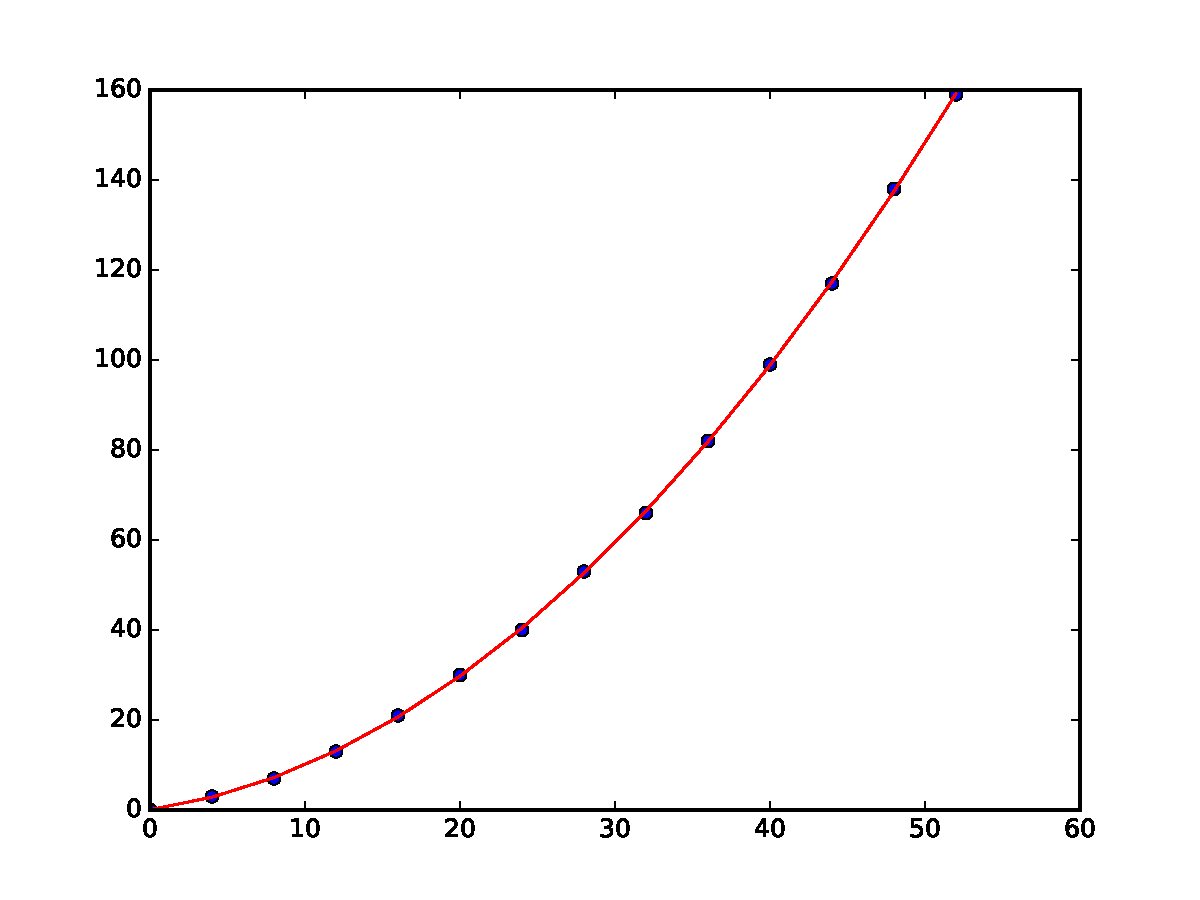
\includegraphics[width=10cm]{./Echolesky_1.pdf}
 % Echolesky_1.pdf: 0x0 pixel, 300dpi, 0.00x0.00 cm, bb=
 \caption{Validation graphique}
 \label{fig: Echolesky_2}
\end{figure}

